% Created by tikzDevice version 0.8.1 on 2015-03-29 20:56:35
% !TEX encoding = UTF-8 Unicode
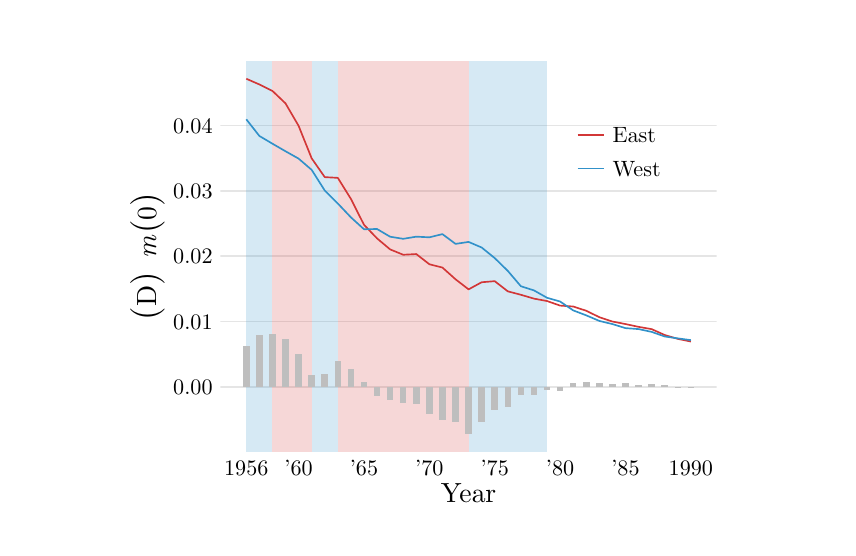
\begin{tikzpicture}[x=1pt,y=1pt]
\definecolor{fillColor}{RGB}{255,255,255}
\path[use as bounding box,fill=fillColor,fill opacity=0.00] (0,0) rectangle (289.08,180.67);
\begin{scope}
\path[clip] ( 28.06,  0.00) rectangle (261.02,180.67);

\path[] ( 28.06,  0.00) rectangle (261.02,180.68);
\end{scope}
\begin{scope}
\path[clip] ( 69.66, 27.29) rectangle (248.98,168.63);

\path[] ( 69.66, 27.29) rectangle (248.98,168.63);
\definecolor{drawColor}{gray}{0.90}

\path[draw=drawColor,line width= 0.6pt,line join=round] ( 69.66, 50.85) --
	(248.98, 50.85);

\path[draw=drawColor,line width= 0.6pt,line join=round] ( 69.66, 74.47) --
	(248.98, 74.47);

\path[draw=drawColor,line width= 0.6pt,line join=round] ( 69.66, 98.10) --
	(248.98, 98.10);

\path[draw=drawColor,line width= 0.6pt,line join=round] ( 69.66,121.72) --
	(248.98,121.72);

\path[draw=drawColor,line width= 0.6pt,line join=round] ( 69.66,145.35) --
	(248.98,145.35);
\definecolor{fillColor}{RGB}{49,145,201}

\path[fill=fillColor,fill opacity=0.20] ( 79.00, 27.29) rectangle ( 88.45,168.63);
\definecolor{fillColor}{RGB}{210,55,55}

\path[fill=fillColor,fill opacity=0.20] ( 88.45, 27.29) rectangle (102.62,168.63);
\definecolor{fillColor}{RGB}{49,145,201}

\path[fill=fillColor,fill opacity=0.20] (102.62, 27.29) rectangle (112.07,168.63);
\definecolor{fillColor}{RGB}{210,55,55}

\path[fill=fillColor,fill opacity=0.20] (112.07, 27.29) rectangle (159.32,168.63);
\definecolor{fillColor}{RGB}{49,145,201}

\path[fill=fillColor,fill opacity=0.20] (159.32, 27.29) rectangle (187.67,168.63);
\definecolor{drawColor}{RGB}{210,55,55}

\path[draw=drawColor,line width= 0.6pt,line join=round] ( 79.00,162.21) --
	( 83.72,160.15) --
	( 88.45,157.81) --
	( 93.17,153.31) --
	( 97.90,145.19) --
	(102.62,133.45) --
	(107.35,126.66) --
	(112.07,126.40) --
	(116.80,118.79) --
	(121.52,109.45) --
	(126.25,104.52) --
	(130.97,100.55) --
	(135.70, 98.61) --
	(140.42, 98.87) --
	(145.15, 95.18) --
	(149.87, 93.99) --
	(154.60, 89.75) --
	(159.32, 86.11) --
	(164.05, 88.68) --
	(168.77, 89.07) --
	(173.50, 85.39) --
	(178.22, 84.15) --
	(182.95, 82.76) --
	(187.67, 81.89) --
	(192.40, 80.24) --
	(197.12, 79.91) --
	(201.85, 78.37) --
	(206.57, 76.05) --
	(211.30, 74.48) --
	(216.02, 73.57) --
	(220.75, 72.56) --
	(225.47, 71.74) --
	(230.20, 69.61) --
	(234.92, 68.22) --
	(239.65, 67.25);
\definecolor{drawColor}{RGB}{49,145,201}

\path[draw=drawColor,line width= 0.6pt,line join=round] ( 79.00,147.56) --
	( 83.72,141.54) --
	( 88.45,138.74) --
	( 93.17,136.01) --
	( 97.90,133.35) --
	(102.62,129.29) --
	(107.35,121.82) --
	(112.07,117.13) --
	(116.80,112.13) --
	(121.52,107.84) --
	(126.25,107.91) --
	(130.97,105.13) --
	(135.70,104.37) --
	(140.42,105.15) --
	(145.15,104.91) --
	(149.87,106.07) --
	(154.60,102.54) --
	(159.32,103.25) --
	(164.05,101.23) --
	(168.77, 97.40) --
	(173.50, 92.77) --
	(178.22, 87.23) --
	(182.95, 85.73) --
	(187.67, 83.07) --
	(192.40, 81.71) --
	(197.12, 78.51) --
	(201.85, 76.71) --
	(206.57, 74.70) --
	(211.30, 73.56) --
	(216.02, 72.10) --
	(220.75, 71.75) --
	(225.47, 70.74) --
	(230.20, 69.08) --
	(234.92, 68.40) --
	(239.65, 67.76);
\definecolor{fillColor}{RGB}{190,190,190}

\path[fill=fillColor] ( 77.81, 50.85) rectangle ( 80.18, 65.49);

\path[fill=fillColor] ( 82.54, 50.85) rectangle ( 84.90, 69.46);

\path[fill=fillColor] ( 87.26, 50.85) rectangle ( 89.63, 69.92);

\path[fill=fillColor] ( 91.99, 50.85) rectangle ( 94.35, 68.14);

\path[fill=fillColor] ( 96.71, 50.85) rectangle ( 99.08, 62.69);

\path[fill=fillColor] (101.44, 50.85) rectangle (103.80, 55.00);

\path[fill=fillColor] (106.16, 50.85) rectangle (108.53, 55.69);

\path[fill=fillColor] (110.89, 50.85) rectangle (113.25, 60.12);

\path[fill=fillColor] (115.61, 50.85) rectangle (117.98, 57.51);

\path[fill=fillColor] (120.34, 50.85) rectangle (122.70, 52.46);

\path[fill=fillColor] (125.06, 47.46) rectangle (127.43, 50.85);

\path[fill=fillColor] (129.79, 46.27) rectangle (132.15, 50.85);

\path[fill=fillColor] (134.51, 45.08) rectangle (136.88, 50.85);

\path[fill=fillColor] (139.24, 44.57) rectangle (141.60, 50.85);

\path[fill=fillColor] (143.96, 41.12) rectangle (146.33, 50.85);

\path[fill=fillColor] (148.69, 38.77) rectangle (151.05, 50.85);

\path[fill=fillColor] (153.41, 38.06) rectangle (155.78, 50.85);

\path[fill=fillColor] (158.14, 33.71) rectangle (160.50, 50.85);

\path[fill=fillColor] (162.86, 38.30) rectangle (165.23, 50.85);

\path[fill=fillColor] (167.59, 42.52) rectangle (169.95, 50.85);

\path[fill=fillColor] (172.31, 43.46) rectangle (174.68, 50.85);

\path[fill=fillColor] (177.04, 47.76) rectangle (179.40, 50.85);

\path[fill=fillColor] (181.76, 47.88) rectangle (184.13, 50.85);

\path[fill=fillColor] (186.49, 49.67) rectangle (188.85, 50.85);

\path[fill=fillColor] (191.21, 49.38) rectangle (193.58, 50.85);

\path[fill=fillColor] (195.94, 50.85) rectangle (198.30, 52.25);

\path[fill=fillColor] (200.66, 50.85) rectangle (203.03, 52.51);

\path[fill=fillColor] (205.39, 50.85) rectangle (207.75, 52.19);

\path[fill=fillColor] (210.11, 50.85) rectangle (212.48, 51.77);

\path[fill=fillColor] (214.84, 50.85) rectangle (217.20, 52.32);

\path[fill=fillColor] (219.56, 50.85) rectangle (221.93, 51.66);

\path[fill=fillColor] (224.29, 50.85) rectangle (226.65, 51.85);

\path[fill=fillColor] (229.01, 50.85) rectangle (231.38, 51.37);

\path[fill=fillColor] (233.74, 50.68) rectangle (236.10, 50.85);

\path[fill=fillColor] (238.46, 50.33) rectangle (240.83, 50.85);
\end{scope}
\begin{scope}
\path[clip] (  0.00,  0.00) rectangle (289.08,180.67);
\definecolor{drawColor}{RGB}{0,0,0}

\node[text=drawColor,anchor=base east,inner sep=0pt, outer sep=0pt, scale=  0.80] at ( 66.82, 48.09) {0.00};

\node[text=drawColor,anchor=base east,inner sep=0pt, outer sep=0pt, scale=  0.80] at ( 66.82, 71.72) {0.01};

\node[text=drawColor,anchor=base east,inner sep=0pt, outer sep=0pt, scale=  0.80] at ( 66.82, 95.34) {0.02};

\node[text=drawColor,anchor=base east,inner sep=0pt, outer sep=0pt, scale=  0.80] at ( 66.82,118.97) {0.03};

\node[text=drawColor,anchor=base east,inner sep=0pt, outer sep=0pt, scale=  0.80] at ( 66.82,142.59) {0.04};
\end{scope}
\begin{scope}
\path[clip] (  0.00,  0.00) rectangle (289.08,180.67);
\definecolor{drawColor}{RGB}{0,0,0}

\node[text=drawColor,anchor=base,inner sep=0pt, outer sep=0pt, scale=  0.80] at ( 79.00, 18.93) {1956};

\node[text=drawColor,anchor=base,inner sep=0pt, outer sep=0pt, scale=  0.80] at ( 97.90, 18.93) {'60};

\node[text=drawColor,anchor=base,inner sep=0pt, outer sep=0pt, scale=  0.80] at (121.52, 18.93) {'65};

\node[text=drawColor,anchor=base,inner sep=0pt, outer sep=0pt, scale=  0.80] at (145.15, 18.93) {'70};

\node[text=drawColor,anchor=base,inner sep=0pt, outer sep=0pt, scale=  0.80] at (168.77, 18.93) {'75};

\node[text=drawColor,anchor=base,inner sep=0pt, outer sep=0pt, scale=  0.80] at (192.40, 18.93) {'80};

\node[text=drawColor,anchor=base,inner sep=0pt, outer sep=0pt, scale=  0.80] at (216.02, 18.93) {'85};

\node[text=drawColor,anchor=base,inner sep=0pt, outer sep=0pt, scale=  0.80] at (239.65, 18.93) {1990};
\end{scope}
\begin{scope}
\path[clip] (  0.00,  0.00) rectangle (289.08,180.67);
\definecolor{drawColor}{RGB}{0,0,0}

\node[text=drawColor,anchor=base,inner sep=0pt, outer sep=0pt, scale=  1.00] at (159.32,  9.03) {Year};
\end{scope}
\begin{scope}
\path[clip] (  0.00,  0.00) rectangle (289.08,180.67);
\definecolor{drawColor}{RGB}{0,0,0}

\node[text=drawColor,rotate= 90.00,anchor=base west,inner sep=0pt, outer sep=0pt, scale=  1.25] at ( 46.46, 75.01) {(};

\node[text=drawColor,rotate= 90.00,anchor=base west,inner sep=0pt, outer sep=0pt, scale=  1.00] at ( 46.46, 79.87) {D};

\node[text=drawColor,rotate= 90.00,anchor=base west,inner sep=0pt, outer sep=0pt, scale=  1.25] at ( 46.46, 87.51) {)};

\node[text=drawColor,rotate= 90.00,anchor=base west,inner sep=0pt, outer sep=0pt, scale=  1.00] at ( 46.46, 92.37) { };

\node[text=drawColor,rotate= 90.00,anchor=base west,inner sep=0pt, outer sep=0pt, scale=  1.00] at ( 46.46, 97.37) {\itshape m};

\node[text=drawColor,rotate= 90.00,anchor=base west,inner sep=0pt, outer sep=0pt, scale=  1.25] at ( 46.46,106.19) {(};

\node[text=drawColor,rotate= 90.00,anchor=base west,inner sep=0pt, outer sep=0pt, scale=  1.00] at ( 46.46,111.05) {0};

\node[text=drawColor,rotate= 90.00,anchor=base west,inner sep=0pt, outer sep=0pt, scale=  1.25] at ( 46.46,116.05) {)};
\end{scope}
\begin{scope}
\path[clip] (  0.00,  0.00) rectangle (289.08,180.67);

\path[] (193.23,119.48) rectangle (232.99,161.24);
\end{scope}
\begin{scope}
\path[clip] (  0.00,  0.00) rectangle (289.08,180.67);
\definecolor{drawColor}{RGB}{210,55,55}

\path[draw=drawColor,line width= 0.6pt,line join=round] (198.71,141.82) -- (208.34,141.82);
\end{scope}
\begin{scope}
\path[clip] (  0.00,  0.00) rectangle (289.08,180.67);
\definecolor{drawColor}{RGB}{49,145,201}

\path[draw=drawColor,line width= 0.6pt,line join=round] (198.71,129.77) -- (208.34,129.77);
\end{scope}
\begin{scope}
\path[clip] (  0.00,  0.00) rectangle (289.08,180.67);
\definecolor{drawColor}{RGB}{0,0,0}

\node[text=drawColor,anchor=base west,inner sep=0pt, outer sep=0pt, scale=  0.80] at (211.35,139.06) {East};
\end{scope}
\begin{scope}
\path[clip] (  0.00,  0.00) rectangle (289.08,180.67);
\definecolor{drawColor}{RGB}{0,0,0}

\node[text=drawColor,anchor=base west,inner sep=0pt, outer sep=0pt, scale=  0.80] at (211.35,127.02) {West};
\end{scope}
\end{tikzpicture}
